\scanpage{51}

Sous-algèbres tautologiques de $H^*(X^n)$.

\textcircled{1}\quad\uline{$H^*(X)$}
\deleted{\unsure{degré}}

\uline{générateurs}\quad $\unsure{y|\eta}\in H^{\unsure{n|m}}(X)$

\uline{relations}\quad $\unsure{y|\eta}^2=0$

\uline{base}
\diagram{$
\begin{array}{ll}
\text{deg. }0&1\\
\text{deg. }\unsure{n|m}&\unsure{y|\eta}
\end{array}
$}

\textcircled{2}\quad\uline{$H^*(X\times X)$}

\uline{générateurs}:
\[
\unsure{y|\eta}\otimes1=\unsure{y|\eta}_1\ \deleted{\unsure{*}},\quad
1\otimes\unsure{y|\eta}=\unsure{y|\eta}_2,\quad
\delta\in H^{\unsure{n|m}}(X)
\]

\uline{relations}
\[
\unsure{y|\eta}_1^2=\unsure{y|\eta}_2^2=0,\quad
\unsure{y|\eta}_1\unsure{y|\eta}_2=\unsure{y|\eta}_1\delta=\unsure{y|\eta}_2\delta;\quad
\delta^2=\chi\,\unsure{y|\eta}_1\unsure{y|\eta}_2
\]
\margin{($\chi\in\mathbb Z$ la car. d'EP)}

\uline{base}
\diagram{$
\begin{array}{ll}
\text{deg }0&1\\
\text{deg }\unsure{n|m}&\unsure{y|\eta}_1,\unsure{y|\eta}_2,\delta\\
\text{deg }2\unsure{n|m}&\unsure{y|\eta}_1\unsure{y|\eta}_2\unsure{y|\eta}_3
\end{array}
$}

\textcircled{3}\quad $H^*(X\times X\times X)$

\uline{générateurs}
\[
\begin{array}{ll}
\text{deg. }\unsure{n|m}:&
\unsure{y|\eta}\otimes1\otimes1=\unsure{y|\eta}_1,\quad
1\otimes\unsure{y|\eta}\otimes1=\unsure{y|\eta}_2,\quad
1\otimes1\otimes\unsure{y|\eta}=\unsure{y|\eta}_3,\quad
\delta_{12}=\delta\otimes1,\delta_{23},\delta_{31}\\
\text{deg }2\unsure{n|m}&\delta
\end{array}
\]

\uline{relations}
\[
\left\{
\begin{aligned}
&\unsure{y|\eta}_1^2=\unsure{y|\eta}_2^2=\unsure{y|\eta}_3^2=0\\
&\delta_{12}^2=\chi\unsure{y|\eta}_1\unsure{y|\eta}_2,\quad
\delta_{23}^2=\chi\unsure{y|\eta}_2\unsure{y|\eta}_3,\quad
\delta_{31}^2=\chi\unsure{y|\eta}_3\unsure{y|\eta}_1,\quad
\delta_{12}\delta_{23}=\delta_{12}\delta_{31}=\delta_{23}\delta_{31}=\delta\\
&\delta_{12}\unsure{y|\eta}_1=\delta_{12}\unsure{y|\eta}_2=\deleted{\delta}\unsure{y|\eta}_1\unsure{y|\eta}_2,\quad
\delta_{23}\unsure{y|\eta}_2=\delta_{23}\unsure{y|\eta}_3=\unsure{y|\eta}_2\unsure{y|\eta}_3,\quad
\delta_{31}\unsure{y|\eta}_3=\delta_{31}\unsure{y|\eta}_1=\unsure{y|\eta}_3\unsure{y|\eta}_1,\\
&\delta\unsure{y|\eta}_1=\delta\unsure{y|\eta}_2=\delta\unsure{y|\eta}_3=\unsure{y|\eta}_1\unsure{y|\eta}_2\unsure{y|\eta}_3\\
&\delta^2=0\\
&\delta_{12}\delta=\delta_{23}\delta=\delta_{31}\delta=\chi\unsure{y|\eta}_1\unsure{y|\eta}_2\unsure{y|\eta}_3
\end{aligned}
\right.
\]

\uline{base}
\diagram{$
\begin{array}{ll}
\text{deg }0&1\\
\text{deg }\unsure{n|m}&\unsure{y|\eta}_1,\unsure{y|\eta}_2,\unsure{y|\eta}_3,\delta_{12},\delta_{23},\delta_{31}\\
\text{deg }2\unsure{n|m}&\unsure{y|\eta}_1\unsure{y|\eta}_2,\unsure{y|\eta}_2\unsure{y|\eta}_3,\unsure{y|\eta}_3\unsure{y|\eta}_1,\delta_{12}\unsure{y|\eta}_3,\delta_{23}\unsure{y|\eta}_1,\delta_{31}\unsure{y|\eta}_2,\delta\\
\text{deg }3\unsure{n|m}&\unsure{y|\eta}_1\unsure{y|\eta}_2\unsure{y|\eta}_3
\end{array}
$}
\figure{
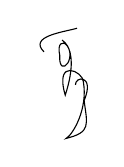
\begin{tikzpicture}[x=1cm,y=1cm]
\draw[thin] (0,1.1) .. controls (-.2,1.3) and (.25,1.35) .. (.42,1.4);
\draw[thin] (.23,1.25) .. controls (.48,1.06) and (.18,.72) .. (.2,1.06)
.. controls (.13,1.35) and (.5,1.25) .. (.27,.55)
.. controls (.13,1.03) and (.5,.85) .. (.5,.72)
.. controls (.56,.38) and (.37,.05) .. (.28,0)
.. controls (.6,.08) and (.55,.17) .. (.51,.48)
.. controls (.65,.82) and (.39,.79) .. (.4,.68);
\end{tikzpicture}
}
\margin{50}
